\documentclass[conference,a4paper]{IEEEtran}
\IEEEoverridecommandlockouts
\usepackage{cite}
\usepackage{amsmath,amssymb,amsfonts}
\usepackage{graphicx}
\usepackage{textcomp}
\usepackage{xcolor}
\usepackage{booktabs}
\usepackage{multirow}
\usepackage{url}
\usepackage{tikz}
\usetikzlibrary{positioning,arrows.meta,fit,backgrounds,calc}
\graphicspath{{figures/}}

% Visible placeholder for facts only the authors can supply. Resolve all before submission:
%   grep -n authortodo main.tex
\newcommand{\authortodo}[1]{\textcolor{red}{\textbf{[TODO: #1]}}}
\newcommand{\R}{\mathbb{R}}

\begin{document}

\title{HyBench3D: A Leakage-free Benchmark of 3D CNN, Transformer, and Hybrid Networks for Alzheimer's Disease Classification in 3D MRI}

\author{
\IEEEauthorblockN{Samuel Emon Halder, Faria Zarin Subah, A.S. Zaforullah Momtaz}
\IEEEauthorblockA{Department of Computer Science and Engineering, University of Asia Pacific, Dhaka, Bangladesh\\
samueldm714@gmail.com, \{fariazarin, zaforullah\}@uap-bd.edu}
}

\maketitle

\begin{abstract}
In this study, we propose HyBench3D, a leakage-free benchmark that evaluates whether hybrid networks combining a three-dimensional convolutional neural network (3D CNN) with a vision transformer (ViT) improve Alzheimer's disease (AD) classification in 3D MRI. The 3D CNN extracts local features of AD-related abnormalities with its inductive bias, while the transformer models long-range relationships among distant brain regions. Many previous studies report accuracies above 95\%, but most of them split data at the level of 2D slices, so that images of the same patient appear in both training and test sets. In HyBench3D, all networks share the same preprocessing, classifier head, and subject-level five-fold splits, and their differences are tested statistically. In this experiment, we used 1{,}132 3D T1-weighted MRI images of 395 subjects from the Alzheimer's Disease Neuroimaging Initiative (ADNI) and compared six networks: 3D DenseNet-121, MedicalNet-pretrained 3D ResNet-18, 3D ViT, Swin Transformer, and two hybrids (CNN--ViT and Swin--ViT). For cognitively normal (CN) versus AD classification, the CNN--ViT hybrid achieved the highest balanced accuracy of $0.806$, but it was statistically indistinguishable from 3D DenseNet-121 ($0.800$, $p=0.54$) while using twice the parameters. Removing the CNN branch decreased the macro-F1 score in all five folds, and an age-and-sex-only baseline remained at chance level. For CN versus mild cognitive impairment (MCI) versus AD classification, the best balanced accuracy was $0.549$ against a chance level of $0.333$. This study demonstrates that, under leakage-free evaluation, the convolutional branch carries the discriminative signal, and the transformer branch adds no measurable value at the scale of a typical ADNI cohort.
\end{abstract}

\begin{IEEEkeywords}
Alzheimer's disease, 3D MRI, 3D CNN, vision transformer, hybrid network, data leakage, explainable AI
\end{IEEEkeywords}

\begin{figure}[t]
\centering
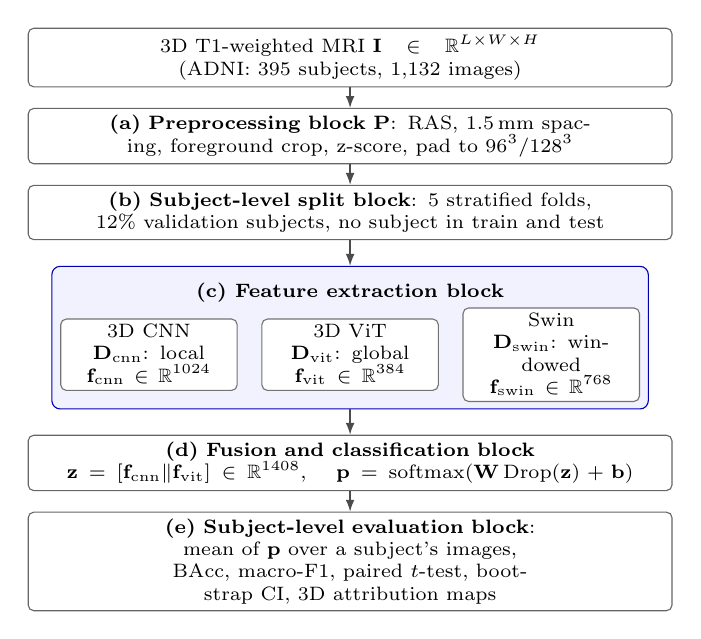
\begin{tikzpicture}[
  font=\scriptsize,
  box/.style={draw=black!60, rounded corners=2pt, align=center, inner sep=2.5pt, fill=white, text width=80mm},
  sub/.style={draw=black!55, rounded corners=2pt, align=center, inner sep=2pt, fill=white, text width=21mm, minimum height=9mm},
  hl/.style={draw=blue!70!black, rounded corners=3pt, fill=blue!5, inner sep=3pt},
  arr/.style={-{Latex[length=1.5mm]}, black!70, line width=0.5pt}]
\node[box] (in) {3D T1-weighted MRI $\mathbf{I}\in\R^{L\times W\times H}$ (ADNI: 395 subjects, 1{,}132 images)};
\node[box, below=2.6mm of in] (pre) {\textbf{(a) Preprocessing block} $\mathbf{P}$: RAS, 1.5\,mm spacing, foreground crop, z-score, pad to $96^3$/$128^3$};
\node[box, below=2.6mm of pre] (split) {\textbf{(b) Subject-level split block}: 5 stratified folds, 12\% validation subjects, no subject in train and test};
\node[font=\scriptsize\bfseries, below=4.2mm of split] (lbl) {(c) Feature extraction block};
\node[sub, below=0.8mm of lbl] (vit) {3D ViT\\$\mathbf{D}_{\mathrm{vit}}$: global\\$\mathbf{f}_{\mathrm{vit}}\in\R^{384}$};
\node[sub, left=3mm of vit] (cnn) {3D CNN\\$\mathbf{D}_{\mathrm{cnn}}$: local\\$\mathbf{f}_{\mathrm{cnn}}\in\R^{1024}$};
\node[sub, right=3mm of vit] (swin) {Swin\\$\mathbf{D}_{\mathrm{swin}}$: windowed\\$\mathbf{f}_{\mathrm{swin}}\in\R^{768}$};
\begin{scope}[on background layer]
\node[hl, fit=(lbl)(cnn)(vit)(swin), inner ysep=2.5pt] (fe) {};
\end{scope}
\node[box, below=3.2mm of fe] (fuse) {\textbf{(d) Fusion and classification block}\\ $\mathbf{z}=[\mathbf{f}_{\mathrm{cnn}}\Vert\mathbf{f}_{\mathrm{vit}}]\in\R^{1408}$, \quad $\mathbf{p}=\mathrm{softmax}(\mathbf{W}\,\mathrm{Drop}(\mathbf{z})+\mathbf{b})$};
\node[box, below=2.6mm of fuse] (eval) {\textbf{(e) Subject-level evaluation block}: mean of $\mathbf{p}$ over a subject's images,\\ BAcc, macro-F1, paired $t$-test, bootstrap CI, 3D attribution maps};
\draw[arr] (in) -- (pre); \draw[arr] (pre) -- (split); \draw[arr] (split) -- (fe);
\draw[arr] (fe) -- (fuse); \draw[arr] (fuse) -- (eval);
\end{tikzpicture}
\caption{The overall framework of HyBench3D. Every network shares blocks (a), (b), (d), and (e); only the backbone in block (c) changes. The hybrid networks concatenate the features of two backbones.}
\label{fig:framework}
\end{figure}

\section{Introduction}
Convolutional neural networks (CNNs) have established a dominant performance in computer vision~\cite{lecun2015deep}, and they have been widely applied to medical image analysis~\cite{litjens2017survey}. For 3D medical images, a 3D CNN can learn native volumetric representations, and densely connected architectures such as DenseNet~\cite{huang2017densely} train efficiently on small cohorts. However, few large 3D databases are available for pretraining~\cite{chen2019med3d}, and 3D networks require large memory and computation. Especially, the strong inductive bias of convolution restricts each layer to a limited receptive field.

Meanwhile, transformer networks~\cite{vaswani2017attention} have been widely used in computer vision. The vision transformer (ViT)~\cite{dosovitskiy2021image} models the relationships among all image patches with self-attention, so its receptive field covers the whole image. ViT is competitive with CNNs on very large databases, but it tends to underperform on small datasets because it lacks the inductive bias of convolution. The Swin Transformer~\cite{liu2021swin,hatamizadeh2021swinunetr} partly restores locality with shifted windows.

To take advantage of both, hybrid networks combining CNN and transformer have been proposed for Alzheimer's disease (AD) classification~\cite{velu2025design,mahim2024unlocking,jang2022m3t}, and many of them report accuracies above 95\%. However, two problems limit the conclusions of these studies. First, many of them split the data at the level of 2D slices, so that slices of the same patient appear in both training and test sets. Yagis \textit{et al.}~\cite{yagis2021effect} showed that, on the same data and network, this data leakage alone raises the accuracy by about 28 points, and more than half of the reviewed CNN studies may suffer from it~\cite{wen2020convolutional,young2025leakage}. Even 3D networks can leak through longitudinal images of the same subject~\cite{rumala2023split}. Second, hybrid networks are rarely compared with equally tuned single networks on identical splits with statistical tests, so the contribution of the fusion itself remains unknown.

\begin{figure}[t]
\centering
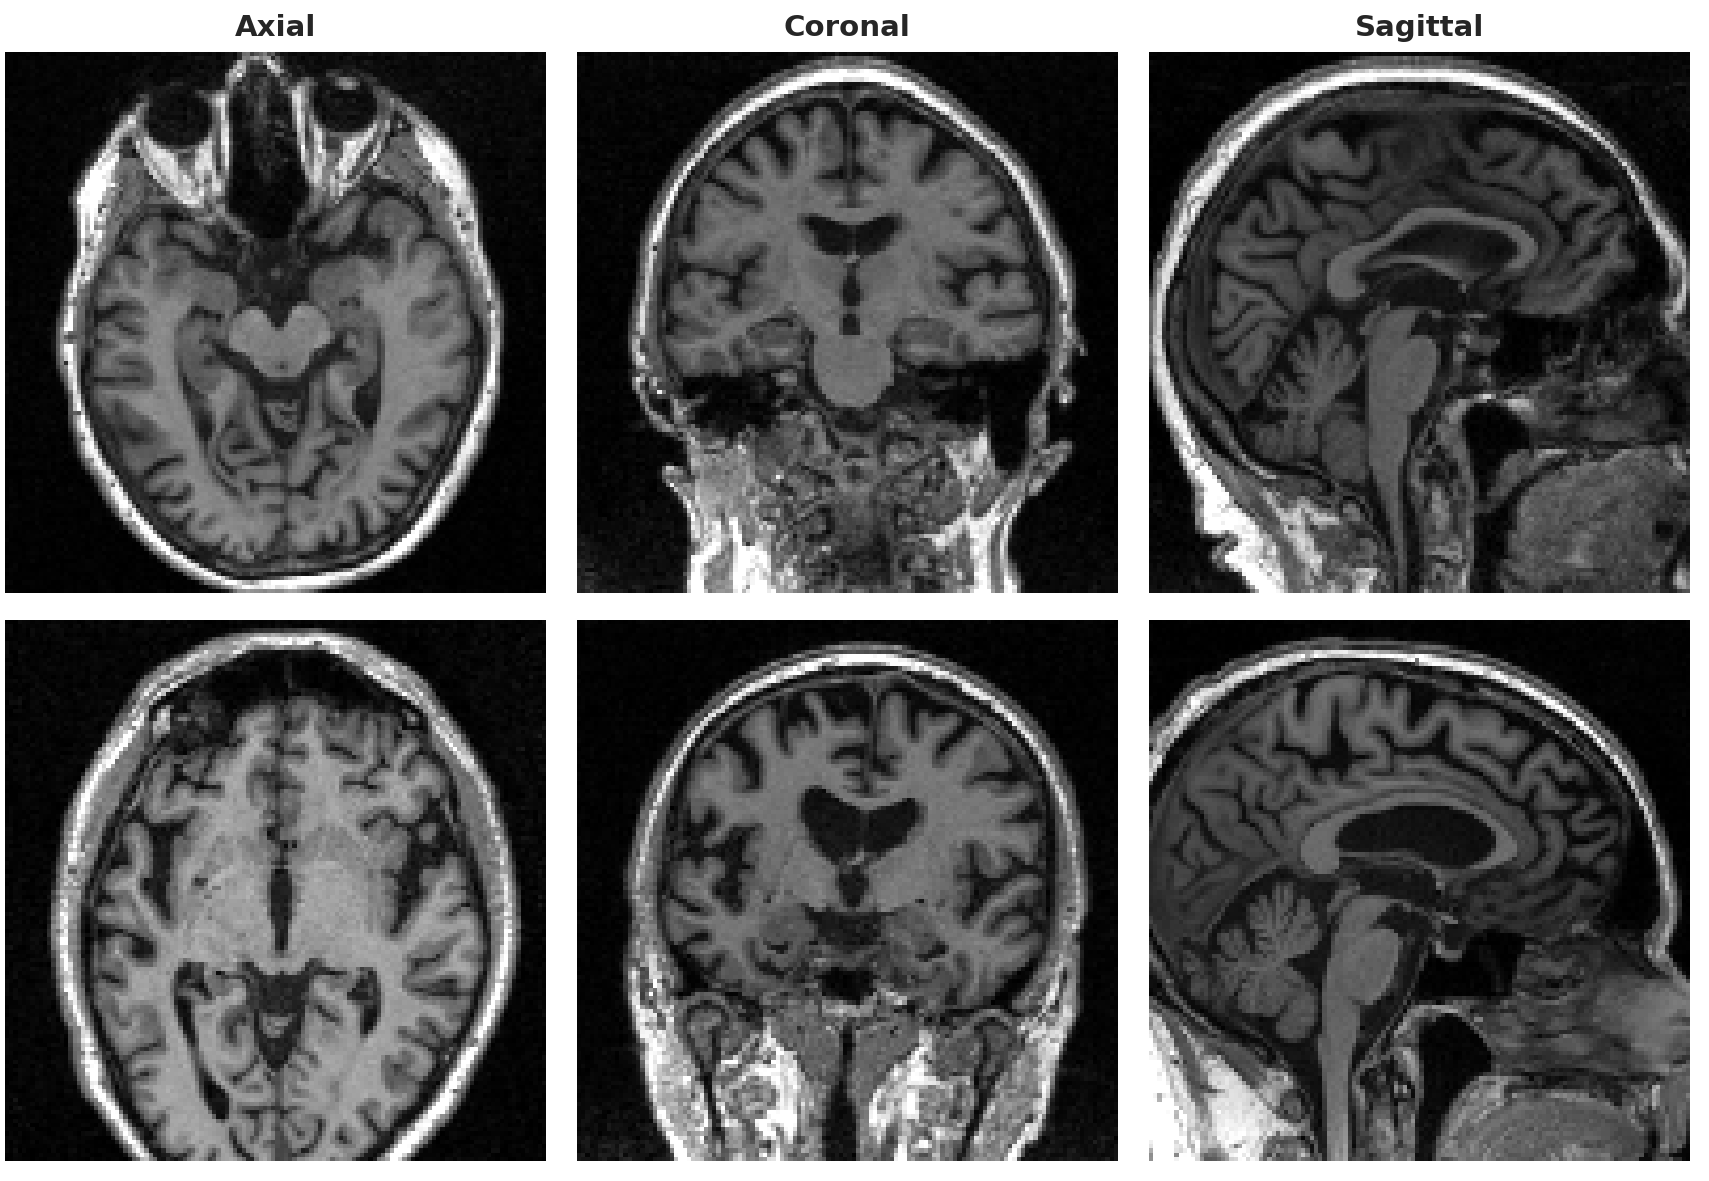
\includegraphics[width=0.76\columnwidth]{fig_cn_ad_samples.png}
\caption{Comparison of a cognitively normal (CN) brain (top) and the structural changes of an Alzheimer's disease (AD) brain (bottom) in axial, coronal, and sagittal planes. The AD brain shows enlarged ventricles and atrophy of the medial temporal lobe.}
\label{fig:samples}
\end{figure}

AD is a progressive neurodegenerative disease that causes memory loss and gradually impairs daily functioning~\cite{scheltens2016alzheimer}. Its progression involves structural changes such as hippocampal shrinkage, ventricular enlargement, and cortical atrophy~\cite{frisoni2010clinical}, which are visible in 3D T1-weighted MRI (Fig.~\ref{fig:samples}). The hippocampal and ventricular changes occur in local regions, which suits a CNN with inductive bias. On the other hand, the cortical atrophy is distributed throughout the brain, which suits a transformer with a wide receptive field. Accordingly, a CNN--transformer hybrid is a natural candidate for AD classification, and the open question is whether it measurably improves on a strong CNN under honest evaluation.

In this study, we propose HyBench3D, a leakage-free benchmark of 3D CNN, transformer, and hybrid networks for AD classification in 3D MRI. Our goal is to measure whether a transformer branch improves a 3D CNN for cognitively normal (CN) versus AD classification and for CN versus mild cognitive impairment (MCI) versus AD classification. The overall framework of HyBench3D is shown in Fig.~\ref{fig:framework}. The main contributions of this study are as follows.

First, HyBench3D evaluates six 3D networks with identical preprocessing, classifier head, imbalance handling, and subject-level splits, and reports majority-class and demographic baselines, fold-paired tests, bootstrap intervals, and network complexity.

Second, through a branch ablation, we show that adding a ViT branch to a 3D CNN doubles the number of parameters (from 11.24M to 23.55M) without a measurable gain ($p=0.54$), whereas replacing the CNN branch decreases the macro-F1 score by 0.14 in every fold.

Third, we report two failure modes that are rarely documented: the instability of a medically pretrained 3D ResNet, and the collapse of a 3D ViT trained from scratch that never predicts the majority class.

Fourth, we visualize the networks with eight 3D attribution methods, show where they disagree, and provide a checklist for evaluating hybrid networks.

\section{Related Works}
\subsection{Transformer and Hybrid Networks for Vision}
SwinUNETR~\cite{hatamizadeh2021swinunetr} extends the shifted-window transformer~\cite{liu2021swin} to 3D medical images. Hybrid networks combine the locality of convolution with the global receptive field of self-attention; for AD, a CNN--Swin hybrid reported 95.34\% on 2D OASIS slices~\cite{velu2025design}, and a ViT--GRU network up to 99.69\%~\cite{mahim2024unlocking}.

\subsection{3D Medical Image Analysis and Data Leakage}
3D CNNs learn volumetric representations directly from MRI volumes~\cite{backstrom2018efficient}, and transfer learning from medical 3D databases is provided by MedicalNet~\cite{chen2019med3d}. However, the evaluation protocol strongly affects the reported performance. Studies that use slice-level splits or curated 2D images report a median accuracy of 99.0\%~\cite{alshayeji2024alzheimer,mahim2024unlocking,el2024novel,alsaeed2022brain,mora2023classification,kurniasari2024transforming,velu2025design,pandey2025leveraging}, whereas studies with subject-level splits report 60--90\%~\cite{wen2020convolutional,saoud2024explainable}. Recent reviews identify data leakage as the most recurrent source of performance inflation in this field~\cite{young2025leakage}.


\subsection{Alzheimer's Disease Classification}
Under subject-level evaluation, Wen \textit{et al.}~\cite{wen2020convolutional} reported 85--88\% for CN versus AD with 3D CNNs, and Saoud and AlMarzouqi~\cite{saoud2024explainable} reported 90\% for CN versus AD and 60\% for the three-class task with an ensemble of 138 regional 3D ViTs. A concurrent study reports 72.3\% on OASIS-1 with a multi-modal 3D CNN~\cite{sifat2026leakage}. M3T~\cite{jang2022m3t} combines 3D and 2D CNNs with a transformer, was trained on 4{,}786 ADNI images, and was tested on independent ADNI, AIBL, and OASIS sets. It reached 93.2\% on ADNI, 1.2 points above a 3D DenseNet-201, from a single run without significance tests. In our work, we focus on whether the transformer branch itself adds value over a matched 3D CNN.

\section{Methods}
\subsection{Overview of HyBench3D}
HyBench3D consists of five main blocks (Fig.~\ref{fig:framework}): 1) a preprocessing block to standardize the 3D MRI images, 2) a subject-level split block to prevent data leakage, 3) a feature extraction block with interchangeable 3D CNN and transformer backbones, 4) a fusion and classification block with a shared head, and 5) a subject-level evaluation block. Only the backbone in block 3) changes between networks.

\subsection{Preprocessing Block}
Given a 3D T1-weighted MRI image $\mathbf{I}$, the preprocessing block $\mathbf{P}$ computes the standardized input $\mathbf{X}$:
\begin{equation}
\mathbf{X}=\mathbf{P}(\mathbf{I})=\mathbf{R}\big(\mathbf{Z}(\mathbf{C}(\mathbf{S}(\mathbf{O}(\mathbf{I}))))\big)\in\R^{L\times W\times H},
\end{equation}
where $\mathbf{O}$ reorients the image to the RAS axes, $\mathbf{S}$ resamples it to $1.5\times1.5\times1.5$\,mm, $\mathbf{C}$ crops the foreground, $\mathbf{Z}$ applies z-score normalization over non-zero voxels, and $\mathbf{R}$ pads or crops it to $L=W=H$. We use $L=128$ for the DenseNet and ResNet networks and $L=96$ for all transformer and hybrid networks. No skull stripping or registration is applied.

\subsection{Subject-level Split Block}
Let $\mathcal{D}=\{(\mathbf{I}_i,y_i,s_i)\}_{i=1}^{N}$ be the images, where $y_i$ is the label and $s_i$ the subject. The subjects are divided into five stratified folds (seed 42), and fold $k$ is tested after training on the remaining folds, so that
\begin{equation}
\{s_i : i\in\mathcal{T}^{\mathrm{train}}_k\}\cap\{s_i : i\in\mathcal{T}^{\mathrm{test}}_k\}=\varnothing .
\end{equation}
Inside each training partition, 12\% of the subjects are held out as a validation set for early stopping and checkpoint selection, so the test fold is never used for model selection.

\subsection{Feature Extraction Block}
Each backbone $\mathbf{D}$ maps $\mathbf{X}$ to a feature vector $\mathbf{f}$. The 3D CNN branch is a DenseNet-121~\cite{huang2017densely} trained from scratch with global average pooling:
\begin{equation}
\mathbf{f}_{\mathrm{cnn}}=\mathbf{D}_{\mathrm{cnn}}(\mathbf{X})\in\R^{1024}.
\end{equation}
The ViT branch~\cite{dosovitskiy2021image} divides $\mathbf{X}$ into $N_p=LWH/p^{3}$ non-overlapping patches of size $p^3$ ($p=16$, $N_p=216$), encodes them with 6 transformer layers (6 heads, hidden size $d=384$, MLP size 1536), and averages the output tokens $\mathbf{T}\in\R^{N_p\times d}$:
\begin{equation}
\mathbf{f}_{\mathrm{vit}}=\frac{1}{N_p}\sum_{n=1}^{N_p}\mathbf{T}_n\in\R^{384}.
\end{equation}
The Swin branch uses the SwinUNETR encoder~\cite{hatamizadeh2021swinunetr} (embedding dimension 48, depths $(2,2,2,2)$, heads $(3,6,12,24)$, window $7^3$) with global average pooling of the deepest stage, $\mathbf{f}_{\mathrm{swin}}\in\R^{768}$. The ResNet-18 branch is initialized with MedicalNet weights~\cite{chen2019med3d}, $\mathbf{f}_{\mathrm{res}}\in\R^{512}$.

\subsection{Fusion and Classification Block}
A hybrid network applies two backbones to the same input and concatenates their features. For the CNN--ViT hybrid,
\begin{equation}
\mathbf{z}=[\mathbf{f}_{\mathrm{cnn}}\,\Vert\,\mathbf{f}_{\mathrm{vit}}]\in\R^{1408},
\end{equation}
and the Swin--ViT hybrid replaces $\mathbf{f}_{\mathrm{cnn}}$ with $\mathbf{f}_{\mathrm{swin}}$. A single network uses $\mathbf{z}=\mathbf{f}$. The shared head computes the class probabilities
\begin{equation}
\mathbf{p}=\mathrm{softmax}\big(\mathbf{W}\,\mathrm{Drop}_{0.2}(\mathbf{z})+\mathbf{b}\big)\in\R^{K},
\end{equation}
where $K=2$ or $3$. For the binary task we use the class-weighted cross-entropy with label smoothing $\epsilon=0.1$~\cite{muller2019does},
\begin{equation}
\ell=-\sum_{c=1}^{K}w_c\,q_c\log p_c,\qquad q_c=(1-\epsilon)\,y_c+\epsilon/K,
\end{equation}
with $w_c=n/(K\,n_c)$, where $n_c$ is the number of training images of class $c$. For the three-class task we use the focal loss~\cite{lin2017focal} $\mathcal{L}=(1-e^{-\ell})^{\gamma}\,\ell$ with $\gamma=2$ and $\epsilon=0$. In addition, every network draws training batches with a class-balanced sampler, $P(i)\propto 1/n_{y_i}$.

\subsection{Subject-level Evaluation Block}
Because a subject contributes 2.9 images on average, the probabilities of its images $I_s=\{i:s_i=s\}$ are averaged:
\begin{equation}
\hat{y}_s=\arg\max_{c}\frac{1}{|I_s|}\sum_{i\in I_s}p_c(\mathbf{I}_i).
\end{equation}
We report the balanced accuracy $\mathrm{BAcc}=\frac{1}{K}\sum_{c}\mathrm{TP}_c/n_c$, the macro-F1 score, accuracy, sensitivity, and specificity (AD as the positive class). Accuracy and macro-F1 are given as mean $\pm$ standard deviation over the five folds, and BAcc with a 95\% subject-level bootstrap confidence interval (10{,}000 resamples). Networks are compared with a paired $t$-test on the fold-wise macro-F1 scores.

\section{Experiments}
\subsection{Experimental Dataset}
In this study, we acquired 3D T1-weighted MPRAGE images from ADNI~\cite{jack2008adni,petersen2010adni} (ADNI GO/2/3, 3T, pre-processed N3m NIfTI). After removing 18 off-protocol images, the dataset contains 1{,}132 images of 395 subjects: 206 CN (627 images), 80 MCI (182), and 109 AD (323). Each subject contributes up to six images acquired within two years (median one year), and each image inherits the ADNI research group of its subject. The groups are matched for age (CN $74.8\pm7.1$, MCI $73.9\pm8.2$, AD $74.7\pm7.9$ years; CN versus AD $p=0.93$) and sex (53\%, 46\%, and 44\% female; $p=0.24$). The ADNI data were collected with the approval of the institutional review boards of the participating sites and are used by authorized investigators under the ADNI Data Use Agreement.

\subsection{Implementation Details}
We implemented HyBench3D with PyTorch~\cite{paszke2019pytorch} and MONAI~\cite{cardoso2022monai}. All networks were trained with the AdamW optimizer~\cite{loshchilov2019decoupled} ($\beta_1=0.9$, $\beta_2=0.999$), linear warmup followed by cosine decay, mixed precision, a batch size of 2 with 4-step gradient accumulation (effective batch size of 8), and gradient clipping at 1.0 on one NVIDIA RTX 5060 Ti GPU (16\,GB). The learning rate is $10^{-4}$, except for the three-class Swin ($5\times10^{-5}$) and the MedicalNet backbone, which is frozen for 5 epochs and then trained at $10^{-5}$. The maximum number of epochs, warmup epochs, early-stopping patience, and weight decay are 80/5/15/0.01 for DenseNet-121, 60/5/12/0.01 for ResNet-18, 100/8/18/0.03 for the hybrids, 100/5/18/0.02 for Swin, and 100/8/18/0.05 for ViT. Training-time augmentation consists of left--right flips, random affine transforms ($\pm10^\circ$, $\pm10\%$ scale, 8-voxel translation), Gaussian noise and smoothing, bias field, gamma ($0.8$--$1.2$), and intensity scaling and shifting.

\subsection{Comparison Study Results}
\begin{table*}[t]
\centering
\caption{Comparison of 3D classification networks for CN versus AD classification (315 subjects). Accuracy and macro-F1: mean $\pm$ SD over five subject-level folds. BAcc, sensitivity (Sens.), and specificity (Spec.): pooled out-of-fold predictions with a 95\% bootstrap CI. Params and GFLOPs: measured for one input volume.}
\label{tab:binary}
\setlength{\tabcolsep}{4.5pt}
\begin{tabular}{lcccccccc}
\toprule
Model name & Input & Params & GFLOPs & Accuracy & Macro-F1 & BAcc [95\% CI] & Sens. & Spec. \\
\midrule
3D DenseNet-121 & $128^3$ & 11.24M & 85.8 & 0.810$\pm$0.041 & 0.788$\pm$0.062 & 0.800 [0.752, 0.846] & \textbf{0.771} & 0.830 \\
3D ResNet-18 (MedicalNet) & $128^3$ & 32.99M & 501.6 & 0.698$\pm$0.139 & 0.654$\pm$0.168 & 0.689 [0.635, 0.742] & 0.670 & 0.709 \\
Swin--ViT hybrid & $96^3$ & 20.37M$^{\dagger}$ & 55.5$^{\dagger}$ & 0.702$\pm$0.070 & 0.662$\pm$0.101 & 0.670 [0.615, 0.724] & 0.569 & 0.772 \\
CNN--ViT hybrid & $96^3$ & 23.55M & 41.9 & \textbf{0.822}$\pm$0.057 & \textbf{0.802}$\pm$0.062 & \textbf{0.806} [0.757, 0.852] & 0.752 & \textbf{0.859} \\
\midrule
\textit{Age + sex only (logistic)} & -- & -- & -- & \textit{0.498}$\pm$\textit{0.092} & \textit{0.486}$\pm$\textit{0.092} & \textit{0.503}$^{\ddagger}$ & -- & -- \\
\textit{Majority class (always CN)} & -- & -- & -- & \textit{0.654} & \textit{0.395} & \textit{0.500} & \textit{0.000} & \textit{1.000} \\
\bottomrule
\end{tabular}
\\[2pt]{\scriptsize $^{\dagger}$Released concatenation variant; the reported run used an earlier ViT branch with extra cross-attention. $^{\ddagger}$Mean over folds.}
\end{table*}

The quantitative performance for CN versus AD classification is presented in Table~\ref{tab:binary}. The CNN--ViT hybrid achieves the highest accuracy (0.822), macro-F1 (0.802), BAcc (0.806), and specificity (0.859). However, the 95\% confidence interval of its BAcc almost coincides with that of 3D DenseNet-121 (0.752--0.846), which achieves a similar performance with less than half the parameters (11.24M versus 23.55M). The Swin--ViT hybrid and the pretrained ResNet-18 are about 12 points lower and much less stable, and the age-and-sex-only classifier remains at chance level, so the networks do not exploit demographic shortcuts.

\begin{table}[t]
\centering
\caption{Comparison of networks for CN versus MCI versus AD classification (395 subjects). Chance-level BAcc is 0.333.}
\label{tab:3class}
\setlength{\tabcolsep}{2.1pt}
\footnotesize
\begin{tabular}{lcccc}
\toprule
Model name & Params & Macro-F1 & BAcc [95\% CI] & MCI recall \\
\midrule
3D DenseNet-121 & 11.25M & 0.524$\pm$0.071 & 0.537 [0.485, 0.588] & \textbf{0.400} \\
Swin & 8.06M & \textbf{0.537}$\pm$0.078 & \textbf{0.549} [0.499, 0.601] & 0.375 \\
3D ViT (scratch) & 12.30M & 0.256$\pm$0.012 & 0.409 [0.363, 0.454] & 0.713 \\
\midrule
\textit{Age + sex only} & -- & \textit{0.371}$\pm$\textit{0.018} & \textit{0.380} & -- \\
\textit{Majority class} & -- & \textit{0.229} & \textit{0.333} & \textit{0.000} \\
\bottomrule
\end{tabular}
\end{table}

For CN versus MCI versus AD classification (Table~\ref{tab:3class}), Swin and 3D DenseNet-121 are statistically tied ($p=0.52$) at a BAcc of about 0.54--0.55, which is clearly above chance. The per-class F1 score is about 0.65 for CN and 0.55--0.61 for AD, but only 0.37--0.41 for MCI. As shown in Fig.~\ref{fig:folds}(b)--(c), most MCI subjects are classified as CN or AD, which is consistent with the clinically intermediate nature of MCI. On the other hand, the 3D ViT trained from scratch never predicts CN (Fig.~\ref{fig:folds}(d)), so its high MCI recall is an artifact rather than evidence of skill. The pure transformer cannot learn meaningful representations from a few hundred subjects~\cite{dosovitskiy2021image}, and the double imbalance correction pushes it toward the minority classes.

\begin{figure*}[t]
\centering
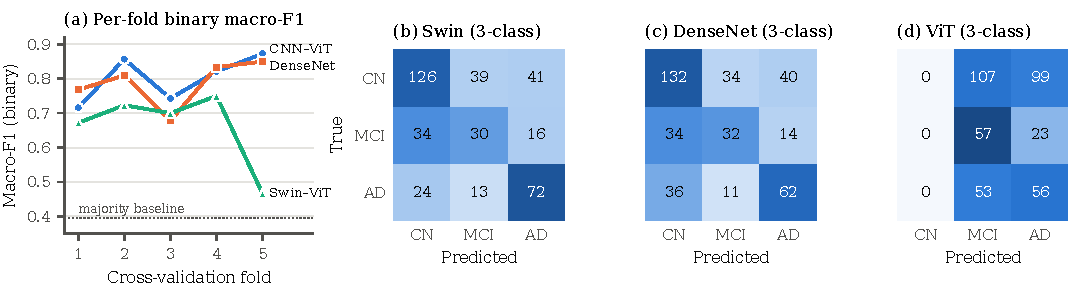
\includegraphics[width=\textwidth]{fig_folds_confusion.pdf}
\caption{(a) Fold-wise macro-F1 for CN versus AD classification on identical subject-level folds: the CNN--ViT hybrid and 3D DenseNet-121 alternate, whereas the Swin--ViT hybrid without a CNN branch is lower in every fold. (b)--(d) Pooled three-class confusion matrices (subject counts; shading is row-normalized).}
\label{fig:folds}
\end{figure*}

\subsection{Ablation Study Results}
To evaluate the degree to which each branch of the CNN--ViT hybrid affects the performance, we compared it with two networks: 1) the hybrid without the ViT branch, which is 3D DenseNet-121, and 2) the hybrid with the CNN branch replaced by Swin, which is the Swin--ViT hybrid. Table~\ref{tab:ablation} shows the results.

\begin{table}[t]
\centering
\caption{Ablation of the CNN--ViT hybrid for CN versus AD classification. $\Delta$: fold-paired difference in macro-F1 from the full hybrid.}
\label{tab:ablation}
\setlength{\tabcolsep}{3pt}
\footnotesize
\begin{tabular}{lccccc}
\toprule
Model & Params & Macro-F1 & $\Delta$ & $p$ & Folds lost \\
\midrule
w/o ViT branch & 11.24M & 0.788 & $-0.014$ & 0.54 & 3/5 \\
CNN branch $\rightarrow$ Swin & 20.37M & 0.662 & $-0.140$ & 0.11 & 5/5 \\
CNN--ViT (full) & 23.55M & \textbf{0.802} & -- & -- & -- \\
\bottomrule
\end{tabular}
\end{table}

Removing the ViT branch reduces the macro-F1 score by only 0.014. The paired $t$-test gives $t=0.67$ with 4 degrees of freedom ($p=0.54$), and the full hybrid classifies 259 of the 315 subjects correctly, against 255 for the CNN alone. On the other hand, replacing the CNN branch with Swin reduces the macro-F1 score by 0.140 and loses in all five folds (Fig.~\ref{fig:folds}(a)). The $t$-test is not significant because of one extreme fold ($p=0.11$), but the BAcc confidence intervals do not overlap (0.615--0.724 versus 0.757--0.852). The convolutional branch therefore carries most of the signal, although input size and schedule also differ, so this is not a strict single-factor ablation. In addition, the MedicalNet-pretrained ResNet-18 is bimodal across folds (three folds reach 0.78--0.82 macro-F1 and two fall to 0.449). Its frozen-backbone start, $10\times$ lower backbone learning rate, and short patience of 12 epochs make a premature early stop likely, although we have not yet confirmed this with a minimum-epoch guard.

\subsection{Visualization Results}
\begin{figure*}[t]
\centering
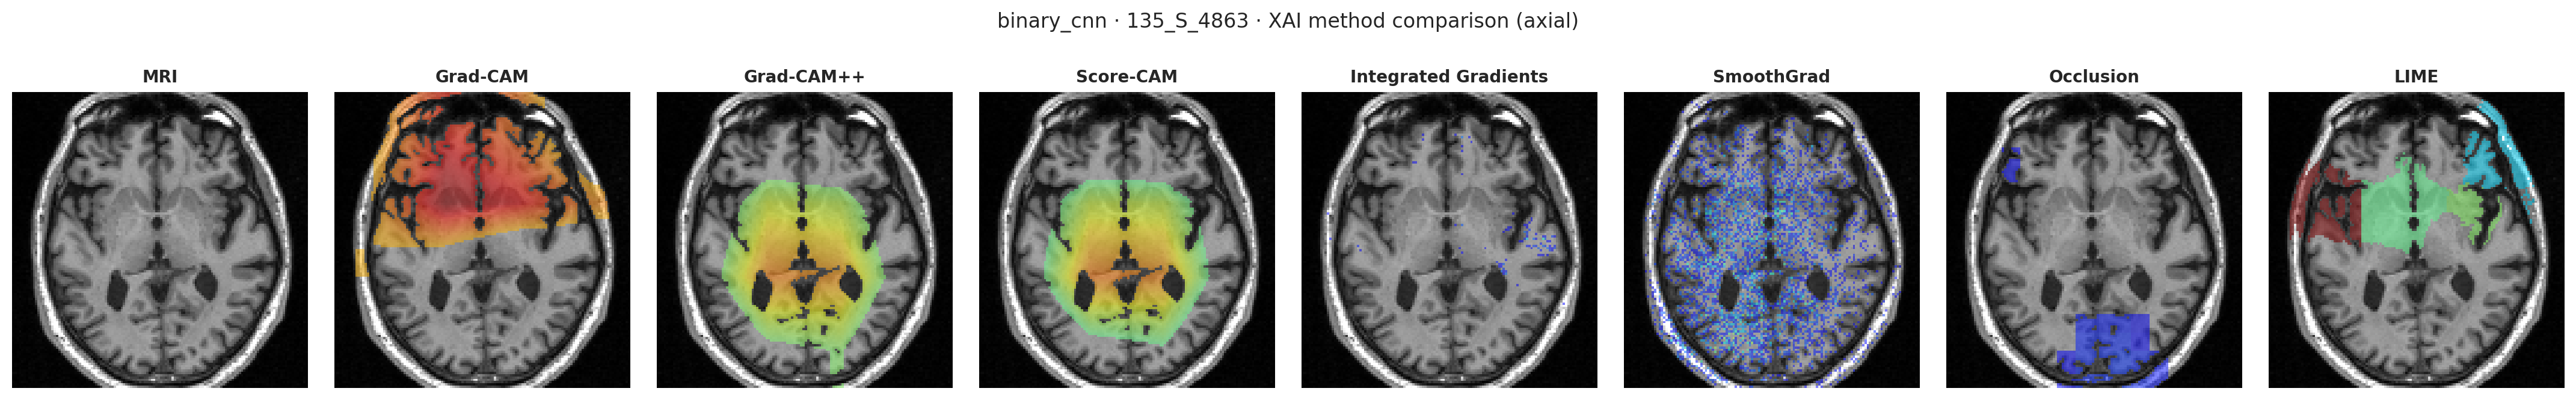
\includegraphics[width=\textwidth]{xai_panel_binary_cnn.png}
\caption{Visualization results of eight 3D attribution methods for 3D DenseNet-121 on one AD subject (axial slice). Grad-CAM focuses on the frontal region, Grad-CAM++ and Score-CAM on the central region, occlusion on the occipital region and posterior skull, and LIME partly on the scalp.}
\label{fig:xai}
\end{figure*}

We visualize the decisions of the networks with Grad-CAM~\cite{selvaraju2017gradcam}, Grad-CAM++~\cite{chattopadhay2018gradcampp}, Score-CAM, Integrated Gradients~\cite{sundararajan2017axiomatic}, SmoothGrad~\cite{smilkov2017smoothgrad}, occlusion, LIME~\cite{ribeiro2016why}, and attention rollout~\cite{abnar2020quantifying}. Fig.~\ref{fig:xai} shows that, on the same subject, the methods highlight different regions. For the Swin and Swin--ViT networks, the Integrated Gradients averaged over 16 AD subjects is nearly uniform across thirds of the volume (0.036--0.055), with mass on the cerebellum, orbits, and scalp rather than a medial-temporal focus. Similar shortcut cues have been reported for 3D MRI networks~\cite{rumala2023split}. Therefore, without skull stripping and atlas registration, the attribution maps cannot confirm that the networks rely on AD-specific anatomy.

\section{Discussion}
Our results lie in the same regime as other subject-level studies: 82\% for CN versus AD against 85--90\%~\cite{wen2020convolutional,saoud2024explainable}, and 58\% for three classes against 60\%~\cite{saoud2024explainable}; the gap is plausibly due to our minimal preprocessing and $96^3$ input. The baseline table of M3T~\cite{jang2022m3t} points in the same direction as our ablation: with four times our training data, adding a transformer to DenseNet-201 \emph{lowered} the ADNI accuracy from 92.0\% to 90.4\%, and a pure 3D ViT was again the weakest network.

We therefore recommend the following checklist for hybrid networks: 1) split at the subject level; 2) report majority-class, chance, and demographic baselines; 3) compare a hybrid with each of its branches on identical folds; 4) use fold-paired tests and confidence intervals; 5) report fold-wise results; and 6) skull-strip inputs and use several attribution methods before anatomical claims.

This study has the following limitations. Standalone ViT and Swin were not trained for the binary task, and the CNN--ViT hybrid was not trained for the three-class task. The results come from a single seed and five folds, so a small benefit of hybridization cannot be ruled out. The labels are the ADNI enrolment groups, applied to images acquired within two years. Finally, the networks were evaluated only on ADNI.

\section{Conclusion}
In this paper, we proposed HyBench3D, a leakage-free benchmark of 3D CNN, transformer, and hybrid networks for AD classification in 3D MRI. Experimental results show that the CNN--ViT hybrid achieves the highest scores for CN versus AD classification, but it is statistically indistinguishable from a 3D CNN with half the parameters, whereas removing the CNN branch consistently decreases the performance. The three-class task is limited by MCI, and the pure 3D ViT fails without pretraining. The visualization results show that attribution maps on non-skull-stripped images are not anatomically conclusive. In future work, we will complete the network grid with repeated cross-validation, add skull stripping and atlas-based attribution, and validate the networks on independent cohorts such as AIBL and OASIS.

\section*{Code Availability}
The code, configurations, and subject-level split files are available at \url{https://github.com/SamuelCormaken/Deep-Learning-for-Alzheimers-MRI}. The ADNI images must be obtained from ADNI under its Data Use Agreement.

\section*{Acknowledgment}
{\footnotesize The authors used Anthropic Claude Sonnet 4.6 solely to check the grammar of the manuscript. All output was reviewed and approved by the authors, who take full responsibility for the content.}

{\footnotesize Data collection and sharing for this project was funded by the Alzheimer's Disease Neuroimaging Initiative (ADNI) (National Institutes of Health Grant U01 AG024904) and DOD ADNI (Department of Defense award number W81XWH-12-2-0012). ADNI is funded by the National Institute on Aging, the National Institute of Biomedical Imaging and Bioengineering, and through generous contributions from the following: AbbVie, Alzheimer's Association; Alzheimer's Drug Discovery Foundation; Araclon Biotech; BioClinica, Inc.; Biogen; Bristol-Myers Squibb Company; CereSpir, Inc.; Cogstate; Eisai Inc.; Elan Pharmaceuticals, Inc.; Eli Lilly and Company; EuroImmun; F. Hoffmann-La Roche Ltd and its affiliated company Genentech, Inc.; Fujirebio; GE Healthcare; IXICO Ltd.; Janssen Alzheimer Immunotherapy Research \& Development, LLC.; Johnson \& Johnson Pharmaceutical Research \& Development LLC.; Lumosity; Lundbeck; Merck \& Co., Inc.; Meso Scale Diagnostics, LLC.; NeuroRx Research; Neurotrack Technologies; Novartis Pharmaceuticals Corporation; Pfizer Inc.; Piramal Imaging; Servier; Takeda Pharmaceutical Company; and Transition Therapeutics. The Canadian Institutes of Health Research is providing funds to support ADNI clinical sites in Canada. Private sector contributions are facilitated by the Foundation for the National Institutes of Health (www.fnih.org). The grantee organization is the Northern California Institute for Research and Education, and the study is coordinated by the Alzheimer's Therapeutic Research Institute at the University of Southern California. ADNI data are disseminated by the Laboratory for Neuro Imaging at the University of Southern California.}

\vspace{2pt}
\noindent{\footnotesize Data used in preparation of this article were obtained from the Alzheimer's Disease Neuroimaging Initiative (ADNI) database (adni.loni.usc.edu). As such, the investigators within the ADNI contributed to the design and implementation of ADNI and/or provided data but did not participate in analysis or writing of this report. A complete listing of ADNI investigators can be found at: \url{http://adni.loni.usc.edu/wp-content/uploads/how_to_apply/ADNI_Acknowledgement_List.pdf}}

\renewcommand{\IEEEbibitemsep}{0pt plus 0.5pt}
\bibliographystyle{IEEEtran}
\bibliography{references}

\end{document}
